\chapter{Introducere}

\section{Tema lucr\u{a}rii}

Inima este motorul organismului, organul care ne \c{t}ine \^{i}n via\c{t}\u{a}. Aceasta are rolul de a prelua s\^{a}ngele \^{i}nc\u{a}rcat cu oxigen \c{s}i substan\c{t}e nutritive venite de la plam\^{a}n \c{s}i de a-l pompa spre toate celelalte organe prin aort\u{a} \c{s}i arterele care se desprind din ea. De asemenea, tot inima este cea care prime\c{s}te s\^{a}ngele inc\u{a}rcat cu dioxid de carbon de la toate organele, prin sistemul venos \c{s}i il pompeaz\u{a} spre pl\u{a}m\^{a}ni pentru oxigenare. Acest circuit se repet\u{a} pe tot parcursul vie\c{t}ii far\u{a} a se \^{i}ntrerupe, p\^{a}n\u{a} c\^{a}nd \^{i}nceteaz\u{a} s\u{a} mai bat\u{a} \c{s}i murim ...
\par 
Bolile de inim\u{a} sunt principala cauz\u{a} de deces la nivel mondial, acestea curm\^{a}nd via\c{t}a unui numar mare de persoane. Potrivit medicilor speciali\c{s}ti, num\u{a}rul mare de decese cauzate de bolile cardiovasculare se afl\u{a} \^{i}n direct\u{a} leg\u{a}tur\u{a} cu dificultatea identific\u{a}rii simptomelor, deoarece acestea nu sunt \^{i}ntotdeauna evidente \c{s}i de cele mai multe ori sunt ignorate sau atribuite unei altei afec\c{t}iuni.
\par 
Din fericire, progresul tehnologic din ultimii ani ne-a adus posibilitatea de a crea noi metode mai eficiente de identificare a simptomelor bolilor cardiace, astfel \^{i}nc\^{a}t acestea s\u{a} poat\u{a} fi tratate \^{i}nc\u{a} de la apari\c{t}ia lor. O astfel de metod\u{a} va fi prezentat\u{a} \^{i}n paginile de mai jos. Aceast\u{a} metod\u{a} presupune identificarea bolilor cardiace folosind \^{i}nregistr\u{a}rile RMN (Rezonan\c{t}\u{a} Magnetic\u{a} Nuclear\u{a}) a unei persoane, preprocesarea lor \c{s}i utilizarea unei re\c{t}ele neuronale pentru stabilirea faptului dac\u{a} persoana respectiv\u{a} prezint\u{a} simptome ale bolilor cardiace.

\section{Prezentarea problemei}

Rezonan\c{t}a Magnetic\u{a} Nuclear\u{a} se folose\c{s}te de un c\^{a}mp magnetic \c{s}i de unde de radiofrecven\c{t}\u{a} pentru vizualizarea diferitelor organe \c{s}i \c{t}esuturi ale corpului omenesc. Undele de radiofrecven\c{t}\u{a} sunt apoi traduse \^{i}ntr-o imagine.
\par
Imaginea de mai jos reprezint\u{a} un exemplu de vizualizare pe care RMN-ul \^{i}l face asupra cutiei toratice. Se poate observa foarte clar inima in aceast\u{a} poz\u{a}.

\begin{center}
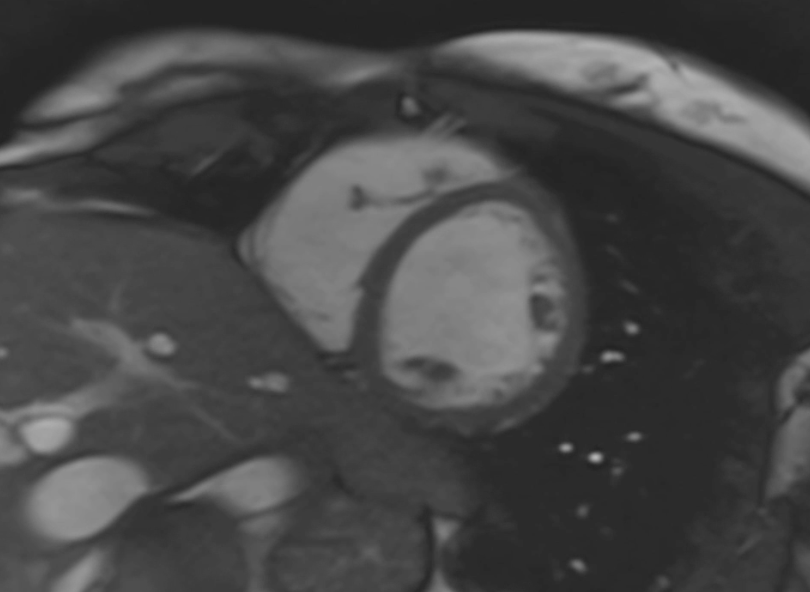
\includegraphics[width=300]{exemple.png}
\end{center}

Cu asemenea tipuri de imagini vom lucra \^{i}n lucrarea de fa\c{t}\u{a} pentru a determina volumul de s\^{a}nge care curge prin ventriculul st\^{a}ng al inimii la dou\u{a} timpuri, dup\u{a} sistol\u{a} c\^{a}nd inima este contractat\u{a} iar prin ventricul curge o cantitate de s\^{a}nge foarte mic\u{a} \c{s}i dup\u{a} diastol\u{a} c\^{a}nd inima este expandat\u{a} iar prin ventricul curge cantitatea cea mai mare de s\^{a}nge.
\par
Dup\u{a} aflarea volumului de s\^{a}nge care curge la sistol\u{a} ( o vom nota cu \textbf{\textit{$V_D$}} ) \c{s}i la diastol\u{a} ( o vom nota cu \textbf{\textit{$V_S$}} ) putem calcula frac\c{t}ia de ejec\c{t}ie a inimii care este definit\u{a} prin urm\u{a}toarea formul\u{a}

$$100 * \frac{V_D - V_S}{V_D}$$

care ne spune proncentajul de s\^{a}nge pe care inima il pompeaz\u{a} prin corp la o b\u{a}taie de a sa.
\par
Pe baza rezultatului ob\c{t}inut de la frac\c{t}ia de ejec\c{t}ie putem stabili dac\u{a} persoana respectiv\u{a} sufera sau nu de o posibil\u{a} boal\u{a} cardiac\u{a}. Dac\u{a} frac\c{t}ia de ejec\c{t}ie este \^{i}ntre 55 \c{s}i 75\%, atunci persoana nu prezint\u{a} posibilitatea de a avea vreo boal\u{a} cardiac\u{a}, ins\u{a} dac\u{a} frac\c{t}ia de ejec\c{t}ie nu se incadreaz\u{a} \^{i}n acel interval atunci persona sufer\u{a} de o boal\u{a} cardiac\u{a}.
\par
\^{I}n mod normal, unui medic specialist \^{i}i ia aproximativ 20 de minute s\u{a} caluleze frac\c{t}ia de ejec\c{t}ie la un pacient pe baza radiografiei RMN. Scopul nostru este acela de a automatiza acest proces, de a-l calcula imediat \c{s}i de a-l face mai accesibil spitalelor, astfle \^{i}nc\^{a}t medicul s\u{a} nu mai fie nevoit s\u{a} efectueze acest proces manual \c{s}i s\u{a} poat\u{a} pune mai repede un diagnostic unui pacient.

\subsection{Datele folosite}

Pentru rezolvarea acestei probleme vom avea desigur nevoie de o cantitate destul de mare de date, \^{i}ns\u{a} acest lucru este rezolvat datorit\u{a} Institutului Na\c{t}ional pentru Inim\u{a}, Pl\u{a}m\^{a}ni \c{s}i S\^{a}nge din America ( The National Heart, Lung, and Blood Institute ), care au pus la dispozi\c{t}ie sute de radiografii RMN ale inimii in format DICOM ( Digital Imaging and Communications in Medicine ), acestea con\c{t}in\^{a}nd aproximativ 30 de cadre care surprind ciclul cardiac al inimii. Acest num\u{a}r poate varia de la caz la caz, imaginile sunt luate din planul perpendicular de-a lungul corpului. Imaginile sunt provenite at\^{a}t de la pacien\c{t}i tineri c\^{a}t \c{s}i de la pacien\c{t}i batr\^{a}ni, pentru c\u{a} bolile inimii pot ap\u{a}rea la orice v\^{a}rst\u{a}, de asemenea imaginile provin de la o multitudine de spitale \c{s}i RMN-uri, astfel c\u{a} calitatea imaginii poate varia.

\par

Varietatea de pozi\c{t}ii prin care un pacient poate sta \^{i}ntr-un RMN, multitudinea de anatomii ale corpului \c{s}i a calit\u{a}\c{t}ii imaginii surprinse de RMN, fac ca m\u{a}surarea cantit\u{a}\c{t}ii de s\^{a}nge care curege prin ventriculul st\^{a}ng al inimii s\u{a} fie o adev\u{a}rat\u{a} provocare.

\section{Imaginea digital\u{a}}

O imagine digital\u{a} este \^{i}mp\u{a}r\c{t}it\u{a} \^{i}n mai multe blocuri infime ca suprafa\c{t}\u{a} numite pixeli. Fiecare pixel are dou\u{a} coordonate care \^{i}i definesc pozi\c{t}ia in imagine \c{s}i o caracteristic\u{a} de luminozitate \c{s}i culoare care este codificat\u{a} conform unui anumit sistem ales. \^{I}n lucrarea de fa\c{t}\u{a} vom folosii sistemul RGB.

\subsection{RGB}

\^{I}n sistemul RGB (Red Green Blue) fiecare pixel este caracterizat prin trei valori, c\^{a}te una pentru fiecare canal, astfle inc\^{a}t valoarea reprezint\u{a} intensitatea pe care pixel-ul o are la un canal. RGB fiind un model aditiv de culoare, \^{i}n care culorile ro\c{s}u, verde \c{s}i albastru sunt amestecate pentru a produce o gam\u{a} larg\u{a} de culori, fiecare valoare a pixel-ului va determina culoarea sa.

\par

\^{I}n sistemul RGB, valoarea pe care un canal o poate lua trebuie s\u{a} fie mai mic\u{a} sau egal\u{a} dec\^{a}t 255 \c{s}i mai mare sau egal\u{a} dec\^{a}t 0. \^{I}n acest tip de reprezentare valoarea 0 este asociat\u{a} culorii negre iar valoarea 255 este asociat\u{a} culorii albe. 

\par

Av\^{a}nd \^{i}n vedere cele scrise mai sus, pentru a reprezenta o culoare \^{i}n sistemul RGB, s\u{a} lu\u{a}m spre exemplu culoarea galben\u{a}, fiecare canal va primii c\^{a}te o valoare din intervalul \^{i}nchis 0 \c{s}i 255, \^{i}n cazul nostru canalul ro\c{s}u va primii valoare 255, canalul verde va primii valoarea 255 iar canalul albastru va primii valoarea 0.

\subsection{Cum vede calculatorul o imagine ?}

Pentru oameni, o imagine este alcatuit\u{a} din obiecte, din peisaje, con\c{t}ine o ac\c{t}iune, un fapt, st\^{a}rne\c{s}te emo\c{t}ii \c{s}i amintiri. Pentru un calculator o imagine este un lung \c{s}ir de numere far\u{a} in\c{t}eles pentru un om din care nu se poate descifra mare lucru. Astfel c\u{a} ne putem pune \^{i}ntrebarea "Cum putem rezolva problema din lucrarea de fa\c{t}\u{a} cu un calculator care nu poate s\u{a} \^{i}n\c{t}eleag\u{a} con\c{t}inutul unei imagini ?". Din fericire exist\u{a} o multitudine de solu\c{t}ii dezvoltate de-a lungul anilor care ne pot ajuta la rezolvarea acestei probleme, \^{i}ns\u{a} cele mai eficiente dintre ele la ora actual\u{a} sunt re\c{t}elele neuronale.

\section{Rezolvarea problemei}

Pentru rezolvarea problemei descrise, aceea de a calcula frac\c{t}ia de ejec\c{t}ie a inimii \^{i}ntr-un mod automat, f\u{a}r\u{a} ajutorul unui om, pe baza c\u{a}reia s\u{a} stabilim dac\u{a} un om are probleme cu inima sau nu \c{s}i dac\u{a} da c\^{a}t de grav este aceasta, propunem cinci pa\c{s}i necesare pentru rezolvarea acestei probleme. Primul pas este de a preprocesa datele furnizate de la Institutul Na\c{t}ional pentru Inim\u{a}, Pl\u{a}m\^{a}ni \c{s}i S\^{a}nge din America. Al doilea pas \^{i}l presupune construirea \c{s}i antrenarea unei re\c{t}ele neuronale convolu\c{t}ionale care s\u{a} primeasc\u{a} imaginile preprocesate \c{s}i s\u{a} fac\u{a} segmentarea ventricului st\^{a}ng al inimii. Al treilea pas va fi calcularea volumului de s\^{a}nge care curge la sistol\u{a} \c{s}i a volumului de s\^{a}nge care curge la diastol\u{a}. Pasul patru este un pas necesar pentru calibrarea datelor calculate la pasul anterior, astfle \^{i}nc\^{a}t calculul volumului de s\^{a}nge care curge la cei doi timpi s\u{a} fie c\^{a}t mai aproape de adev\u{a}r. Ultimul pas va consta \^{i}n calcularea frac\c{t}iei de ejec\c{t}ie pe baza volumelor calculate \c{s}i stabilirea faptului dac\u{a}, pacientul respectiv are sau nu probleme cu inima. 

\par

\^{I}nainte de a trece la partea de implementarea a solu\c{t}iei descrise mai sus, vom face o scurt\u{a} descriere a ceea ce \^{i}nseamn\u{a} o re\c{t}ea neuronalu\u{a}, apoi vom descrie ce este o re\c{t}ea neuronal\u{a} convolu\c{t}ional\u{a}.